\documentclass[11pt,a4paper]{article}

\usepackage[margin=2.5cm]{geometry}
\usepackage{cmap}
\usepackage[T1]{fontenc}
\usepackage{lmodern}
\usepackage{textcomp}
\usepackage{amsmath}
\usepackage{amssymb}
\usepackage{graphicx}
\usepackage{booktabs}
\usepackage{caption}
\usepackage{hyperref}
\usepackage{pdflscape}

\graphicspath{{figures/}{supplementary_media/}}

\captionsetup{labelfont=bf,font=small}
\setlength{\parindent}{0pt}
\setlength{\parskip}{0.65em}

\begin{document}
\begin{center}

{\Large\bfseries Supplementary material for: Motion and Representation Influence Numeriacal-Experimental Agreement in Fish Wake Pressure\par}

\end{center}

\section*{S1. Sample accounting}

The 40 videos, each containing a different fish, were segmented into 493 samples in which the fish was visible. The following table reports all preprocessing categories and whether samples were retained for two-dimensional simulation and pressure comparison. Filtering was completed before simulation and classifier analyses.

\begin{table}[htbp]
\centering
\caption*{Table S1. Accounting of segmented and retained video samples.}
\begin{tabular}{lrrr}
\toprule
Category & Segmented & Retained & Not retained \\
\midrule
Successfully processed & 375 & 367 & 8 \\
Heavy temporal cropping required & 20 & 17 & 3 \\
Poor segmentation & 11 & 6 & 5 \\
No detection in some frames & 26 & 0 & 26 \\
Fish not fully submerged / 3D interaction & 18 & 0 & 18 \\
Fish did not pass in front of sensors & 26 & 0 & 26 \\
Circular segmentation error, tail touching nose & 16 & 13 & 3 \\
External interference, flake in water & 1 & 0 & 1 \\
\midrule
\textbf{Total} & \textbf{493} & \textbf{403} & \textbf{90} \\
\bottomrule
\end{tabular}
\end{table}

\section*{S2. Assessment of fish-identity dependence among retained pressure segments}

Because multiple retained pressure segments could originate from one recording, within-fish dependence was evaluated to determine whether particular individuals might dominate segment-level patterns. Each of the 40 fish appeared in one video, so video identity was equivalent to fish identity. Pressure segments are sensor-specific, so a single retained sample can contribute more than one segment and the segment count exceeds the sample count of Table S1. The measured-pressure diagnostic was restricted to videos with at least five retained pressure segments.

For this diagnostic, measured pressure segments were transformed with the same preprocessing later used for pressure classification and described in the main article: segments were resampled to a common length set by the longest segment in the subset, mean-centred and amplitude-normalised. An SVD basis was then computed from the retained measured-pressure matrix alone, without reference to video labels, and samples were represented by the coefficients of the modes explaining 99\% of measured-signal variance. Video-level dependence was quantified in two complementary ways.

First, a one-way intraclass correlation coefficient, \(\mathrm{ICC}(1)\), was computed separately for each retained SVD mode. For mode \(k\), let \(c_{ij,k}\) be the coefficient of segment \(j=1,\dots,n_i\) from video \(i=1,\dots,G\), where \(n_i\) is the number of segments from video \(i\), \(G\) the number of videos and \(N=\sum_i n_i\). Coefficients were modelled as \(c_{ij,k}=\mu_k+a_{i,k}+\varepsilon_{ij,k}\), in which \(a_{i,k}\) is a random video effect of variance \(\sigma^2_{\mathrm{video},k}\) and \(\varepsilon_{ij,k}\) an independent residual segment effect of variance \(\sigma^2_{\mathrm{segment},k}\). The video and overall coefficient means were
\begin{equation}
\bar c_{i,k}=\frac{1}{n_i}\sum_j c_{ij,k},
\qquad
\bar c_k=\frac{1}{N}\sum_i\sum_j c_{ij,k}.
\end{equation}

Between-video and within-video variation were represented by the one-way analysis-of-variance mean squares
\begin{align}
\mathrm{MS}_{\mathrm{between},k}
&=\frac{\sum_i n_i(\bar c_{i,k}-\bar c_k)^2}{G-1},\\
\mathrm{MS}_{\mathrm{within},k}
&=\frac{\sum_i\sum_j(c_{ij,k}-\bar c_{i,k})^2}{N-G}.
\end{align}
Because videos contained unequal numbers of segments, the effective number of segments per video was
\begin{equation}
n_0=\frac{N-\sum_i n_i^2/N}{G-1}.
\end{equation}
This reduces to the common number of segments per video when all \(n_i\) are equal. The variance components were estimated as
\begin{align}
\widehat{\sigma}^2_{\mathrm{segment},k}
&=\mathrm{MS}_{\mathrm{within},k},\\
\widehat{\sigma}^2_{\mathrm{video},k}
&=\max\left(\frac{\mathrm{MS}_{\mathrm{between},k}-\mathrm{MS}_{\mathrm{within},k}}{n_0},0\right).
\end{align}
Here \(\widehat{\sigma}^2_{\mathrm{video},k}\) estimates the variance of the video effect and \(\widehat{\sigma}^2_{\mathrm{segment},k}\) the residual variance of segments about their own video mean. The estimator of the video component becomes negative whenever the observed between-video mean square falls below the within-video mean square, which happens by chance when video effects are weak, and was therefore truncated at zero. Truncation can only raise the resulting coefficient, so the estimates reported below are conservative with respect to the conclusion that video-level dependence was weak. The per-mode intraclass correlation was
\begin{equation}
\mathrm{ICC}_k = \frac{\widehat{\sigma}^2_{\mathrm{video},k}}{\widehat{\sigma}^2_{\mathrm{video},k} + \widehat{\sigma}^2_{\mathrm{segment},k}}.
\end{equation}
Values close to zero indicate little video-level clustering, while larger values indicate stronger dependence among segments from the same video. The per-mode ICC values were summarised using the variance-weighted mean
\begin{equation}
\overline{\mathrm{ICC}} = \frac{\sum_k \lambda_k \mathrm{ICC}_k}{\sum_k \lambda_k},
\end{equation}
where \(\lambda_k\) is the SVD eigenvalue for mode \(k\). Modes representing more measured-pressure variation therefore contributed more strongly to the summary.

Second, pairwise Euclidean distances in standardised measured-SVD coefficient space were compared between same-video and different-video segment pairs. The ratio between the median same-video and different-video distances provided a descriptive measure of their similarity. Two resampling procedures were applied to the difference \(\Delta\) between the median different-video and median same-video distances. A permutation test reassigned video labels across segments 1000 times, holding the number of segments per video fixed, and returned the one-sided fraction of permutations reaching the observed \(\Delta\). A cluster bootstrap resampled whole videos with replacement 1000 times, treating every draw of a video as a distinct group, and returned the 2.5th and 97.5th percentiles of \(\Delta\). The permutation test asks whether segments group by video at all while the cluster bootstrap asks how stable the size of that grouping is with respect to which videos happened to be recorded.

The measured-pressure video-identity analysis retained 426 segments from 23 videos and projected them onto 37 measured-pressure SVD modes explaining 99.1\% of variance. The variance-weighted \(\mathrm{ICC}(1)\) was 0.058, and the median per-mode \(\mathrm{ICC}(1)\) was 0.019 (range [0; 0.136] with interquartile range [0.005; 0.032]).

In standardised measured-SVD space, the median same-video distance was 7.006 and the median different-video distance was 7.443, giving \(\Delta=0.437\) and a distance ratio of 0.941. No permutation of video labels reached the observed \(\Delta\), giving \(p=0.001\), the smallest value resolvable with 1000 permutations, so same-video segments were closer to one another than chance label assignment would produce. The cluster bootstrap 95\% interval for \(\Delta\) was [\(-0.012\); 0.974] and included zero, so the magnitude of the effect was not stable across the particular set of videos recorded. Both results agree with the variance components: same-video distances were about 6\% smaller than different-video distances, close to the 5.8\% of coefficient variance attributed to video identity. Clustering by video was therefore detectable but weak. Fish identity contributed little to the observed pressure variation, although segments originating from the same source video should not be interpreted as independent biological replicates.

\section*{S3. Dataset composition and dimensionality reduction}

The following table reports the number of retained pressure segments and the size of the reduced bases used for the pressure-signal classifier. Segments were removed if they were too short or numerically divergent. An equal number of fish and cylinder pressure segments was retained to balance classes.


\begin{table}[htbp]
\centering
\caption*{Table S2. Dataset composition and dimensionality reduction for the four simulation configurations. Raw used original contours and $y$-only boundary forcing. Size-constrained applied the first-frame fish profile along the reconstructed spine and retained $y$-only forcing. X-deformation used original contours with both $x$ and $y$ boundary-motion components. Full combined the profile constraint and two-component forcing. Here, $x$ and $y$ are the fixed long and transverse tank axes.}
\resizebox{\textwidth}{!}{%
\begin{tabular}{lllll}
\toprule
 & Raw & Constrained & X-deformation & Full \\
\midrule
Samples (fish/cylinder) & 163/162 & 159/161 & 161/162 & 162/161 \\
Pressure segments extracted & 956/797 & 796/723 & 1009/798 & 702/723 \\
After minimum-length filter & 238/236 & 186/205 & 200/236 & 192/205 \\
After divergence filter & 238/233 & 171/202 & 189/233 & 186/202 \\
Balanced segments & 233/233 & 171/171 & 189/189 & 186/186 \\
Resampled signal length & 682 & 564 & 580 & 573 \\
Modes for 75\% variance & 5 & 5 & 23 & 6 \\
Modes for 95\% variance & 34 & 32 & 92 & 51 \\
Modes for 99\% variance & 103 & 94 & 153 & 114 \\
\bottomrule
\end{tabular}%
}
\end{table}

\section*{S4. Pressure-signal classifier settings}

The pressure-signal classifier was trained after amplitude normalisation, mean-centring, resampling to a common number of points defined by the longest segment in the relevant subset and projection onto SVD modes retaining 75\%, 95\% or 99\% of simulated variance. A separate SVD basis and a separate classifier were fitted for every combination of simulation variant and retained-variance level. Segments were split into training, validation and test subsets in a 70/15/15 ratio. Hyperparameters for a linear classifier with a Mean Square Error loss were selected independently for each combination.

The implementation comprised two consecutive linear layers without an activation function between them. Their composition remained a linear-affine mapping. The reported hidden width parameterised its factorisation but did not introduce a nonlinear decision boundary. This choice maximised interpretability and limited overfitting for the available dataset. Neural-network tooling was retained for optimisation and future extensibility.

\begin{table}[htbp]
\centering
\caption*{Table S3. Hyperparameters selected independently for each model and retained-variance level.}
\resizebox{\textwidth}{!}{%
\begin{tabular}{llllll}
\toprule
Model & Hidden width & Learning rate & Weight decay & Epochs & Batch size \\
\midrule
Raw 75 & 32 & 0.0002 & 0.0002 & 200 & 64 \\
Constrained 75 & 16 & 0.0006 & 0.0005 & 50 & 16 \\
X-deformation 75 & 32 & 0.0002 & 0.0010 & 200 & 64 \\
Full 75 & 32 & 0.0010 & 0.0006 & 200 & 64 \\
Raw 95 & 4 & 0.0003 & 0.0009 & 200 & 64 \\
Constrained 95 & 8 & 0.0009 & 0.0008 & 200 & 64 \\
X-deformation 95 & 4 & 0.0010 & $3.8626 \times 10^{-5}$ & 100 & 64 \\
Full 95 & 16 & 0.0006 & 0.0002 & 50 & 16 \\
Raw 99 & 4 & 0.0010 & 0.0002 & 200 & 64 \\
Constrained 99 & 16 & 0.0010 & 0.0009 & 100 & 16 \\
X-deformation 99 & 32 & 0.0010 & 0.0008 & 200 & 64 \\
Full 99 & 4 & 0.0006 & 0.0006 & 200 & 64 \\
\bottomrule
\end{tabular}%
}
\end{table}

\section*{S5. Pressure-signal classifier performance}

The following accuracies describe how well the classifier separated fish-generated and cylinder-generated simulated pressure signals. These values were used to assess whether the two simulated model classes were distinguishable before measured pressure signals were projected into the same feature spaces.

These values remained moderate rather than near perfect, but this was not unexpected. The fish and cylinder models can generate partially overlapping pressure signatures in some kinematic situations, particularly when the body turns sharply and presents a locally bluff geometry to the sensor. Perfect separability should therefore not be expected from sparse wall-pressure measurements alone.

\begin{table}[htbp]
\centering
\caption*{Table S4. Classification accuracies for the first-stage pressure-signal classifier.}
\resizebox{\textwidth}{!}{%
\begin{tabular}{lllll}
\toprule
 & Raw & Constrained & X-deformation & Full \\
\midrule
Training accuracy (75\%) & 0.67 & 0.68 & 0.75 & 0.67 \\
Validation accuracy (75\%) & 0.69 & 0.65 & 0.81 & 0.82 \\
Test accuracy (75\%) & 0.74 & 0.63 & 0.84 & 0.61 \\
Training accuracy (95\%) & 0.70 & 0.74 & 0.74 & 0.71 \\
Validation accuracy (95\%) & 0.70 & 0.65 & 0.77 & 0.73 \\
Test accuracy (95\%) & 0.76 & 0.65 & 0.84 & 0.57 \\
Training accuracy (99\%) & 0.78 & 0.75 & 0.80 & 0.75 \\
Validation accuracy (99\%) & 0.64 & 0.65 & 0.84 & 0.66 \\
Test accuracy (99\%) & 0.67 & 0.60 & 0.79 & 0.55 \\
\bottomrule
\end{tabular}%
}
\end{table}

The classifier used a segment-level split, so segments associated with the same source video could occur in different subsets. The limited fish/video dependence identified in Section S2 suggests that shared source-video information alone was unlikely to account for the full classification pattern. However, classifier performance on entirely unseen source videos was not directly evaluated.

\section*{S6. Details of contour-size consistency}

The contour extracted from each video frame was treated independently in the original pipeline. Its projected size could therefore fluctuate because of segmentation noise, natural posture variation or out-of-plane motion such as body roll. A contour-size consistency constraint was introduced to test whether regularising these fluctuations improved agreement with measured pressure. The fish centreline, termed the spine, was first estimated from the raw contour by partitioning the body into upper and lower regions of equal area. The spine was then extrapolated at the snout and tail tips. Finally, a fish profile defined from the first video frame was placed along the spine and optimised against the raw detection by minimising the intersection-over-union mismatch.

The size-constrained sequence therefore retained bending of the reconstructed spine while imposing the first-frame profile and contour length. Subsequent simulation stages were unchanged.

\section*{S7. Details of tank-axis deformation in the CFD twin}

The simulation used fixed tank coordinates: $x$ followed the tank's long axis and $y$ its transverse axis. These terms do not denote instantaneous fish-centred axes.

LilyPad describes interaction between the moving body and fluid through functions for body distance and temporal and spatial boundary variation. In the default implementation used as the starting point, moving-boundary forcing was hard-coded to use only the $y$ component. In the raw model, imported contours still placed each boundary point at its correct $x,y$ position in every frame, but local $x$ displacement between frames was not fully included in the boundary velocity communicated to the fluid. The $y$-only implementation was a deliberate first approximation because idealised fish swimming is often represented as progression along the swimming direction with deformation dominated by lateral undulation. Most observed trajectories were also aligned approximately with the tank's $x$ axis. Real trajectories and body motion could depart from this approximation during turns or when the tail tip moved towards or away from the head.

In the updated implementation, boundary velocity was computed directly from contour-point displacement between consecutive time steps. Both $x$ and $y$ components were used, with local averaging over neighbouring boundary nodes. The contour input was unchanged. This allowed apparent longitudinal redistribution, local extension and compression of the projected contour and other secondary in-plane motions to contribute to the simulated flow.

\section*{S8. Distributional analysis of pressure-conditioned vortices}

The vortex analysis used measured-pressure segments evaluated by the first-stage classifier for the x-deformation variant with 95\% of simulated pressure variance retained. At the 0.99 confidence threshold, measured segments classified as fish-like were linked to the corresponding fish-model vortex tracks and measured segments classified as cylinder-like were linked to the corresponding cylinder-model tracks. Undetermined segments were excluded. The resulting descriptors therefore characterise pressure-conditioned subsets and should not be interpreted as distributions of every vortex produced by either model.

The upstream detection procedure was unchanged. Q-criterion maps were smoothed with a Gaussian filter with a standard deviation of one grid cell. Connected regions above $Q=0.002$ were retained when their area was at least six grid cells. Vortex cores within six grid cells of the body or more than 32 grid cells from their nearest sensor were excluded. Only detections marked visible by the occlusion filter were considered. Detections were linked across frames when their cores were separated by no more than three grid cells, with a maximum frame-index separation of eight. Within each pressure segment, a vortex track was retained when it contained at least 10 consecutive valid visible detections assigned to the same sensor. Classes were not balanced.

Seventeen track-level descriptors were calculated: maximum area, mean area, displacement, path length, straightness, duration in detected frames, duration relative to pressure-segment length, mean distance to the body, mean distance to the sensor, maximum speed, mean speed, maximum equivalent-circle radius, mean equivalent-circle radius, maximum core Q-criterion value, mean core Q-criterion value, mean core $x$-position and mean core $y$-position. Straightness was displacement divided by path length. Radius was calculated as $\sqrt{A/\pi}$ from region area.

Three complementary summaries were calculated. First, all retained vortex-track associations were pooled within each pressure-based class. A physical track intersecting more than one sensor-specific pressure segment was represented once in each relevant association. The pooled subset contained 574 fish-model associations representing 551 distinct physical tracks and 65 cylinder-model associations representing 65 distinct physical tracks. Second, track-level descriptors were averaged within pressure segments so that every segment received equal weight. The number of unique vortices, total vortex-frame occupancy, and mean and maximum simultaneous visible-vortex count were calculated for each segment. This level included 88 fish-associated and 15 cylinder-associated segments. Third, segment summaries were averaged within each source video and model class, giving 21 fish-associated and 10 cylinder-associated videos. Cylinder-minus-fish paired differences were calculated for the 10 source videos represented in both groups. Sample counts, medians and interquartile ranges were reported at each analysis level. At the paired-video level each video contributes a single difference, so mean differences and 95\% confidence intervals from Student's $t$-distribution on $n-1=9$ degrees of freedom were also reported.

\begin{landscape}
\begin{table}[p]
\centering
\caption*{Table S5. Pooled pressure-conditioned vortex-track associations. Values are median (interquartile range). Sample sizes are 574 fish associations and 65 cylinder associations except for fish straightness, which was defined for 549 associations with non-zero path length.}
\begin{tabular*}{0.8\linewidth}{@{\extracolsep{\fill}}lcc@{}}
\toprule
Descriptor & Fish & Cylinder \\
\midrule
Mean area (grid cells) & 13.81 (9.39--22.85) & 32.05 (22.93--38.74) \\
Maximum area (grid cells) & 20.00 (13.00--33.00) & 38.00 (28.00--46.00) \\
Mean equivalent radius (grid cells) & 2.088 (1.724--2.681) & 3.180 (2.700--3.508) \\
Maximum equivalent radius (grid cells) & 2.523 (2.034--3.241) & 3.478 (2.985--3.827) \\
Displacement (grid cells) & 8.60 (4.12--13.93) & 8.60 (5.00--11.70) \\
Path length (grid cells) & 10.91 (5.00--18.00) & 11.41 (6.00--16.12) \\
Straightness & 0.825 (0.739--0.934) & 0.784 (0.717--0.863) \\
Duration (frames) & 86.5 (36.0--165.0) & 81.0 (54.0--115.0) \\
Duration / segment length & 0.401 (0.152--0.751) & 0.625 (0.385--0.855) \\
Mean speed (grid cells frame$^{-1}$) & 0.110 (0.079--0.156) & 0.134 (0.103--0.161) \\
Maximum speed (grid cells frame$^{-1}$) & 1.000 (1.000--1.414) & 1.000 (1.000--1.414) \\
Mean core $Q$ & 0.00976 (0.00627--0.01646) & 0.03309 (0.01981--0.04396) \\
Maximum core $Q$ & 0.01599 (0.00946--0.02579) & 0.04239 (0.02516--0.05334) \\
Mean body distance (grid cells) & 32.80 (17.10--54.86) & 34.97 (23.83--54.54) \\
Mean sensor distance (grid cells) & 19.14 (11.38--23.76) & 21.73 (16.19--26.41) \\
Mean core $x$ (grid cells) & 174.64 (149.17--194.69) & 145.68 (128.50--164.97) \\
Mean core $y$ (grid cells) & 73.39 (64.40--75.96) & 68.71 (63.69--72.19) \\
\bottomrule
\end{tabular*}
\end{table}
\end{landscape}

\begin{figure}[p]
\centering
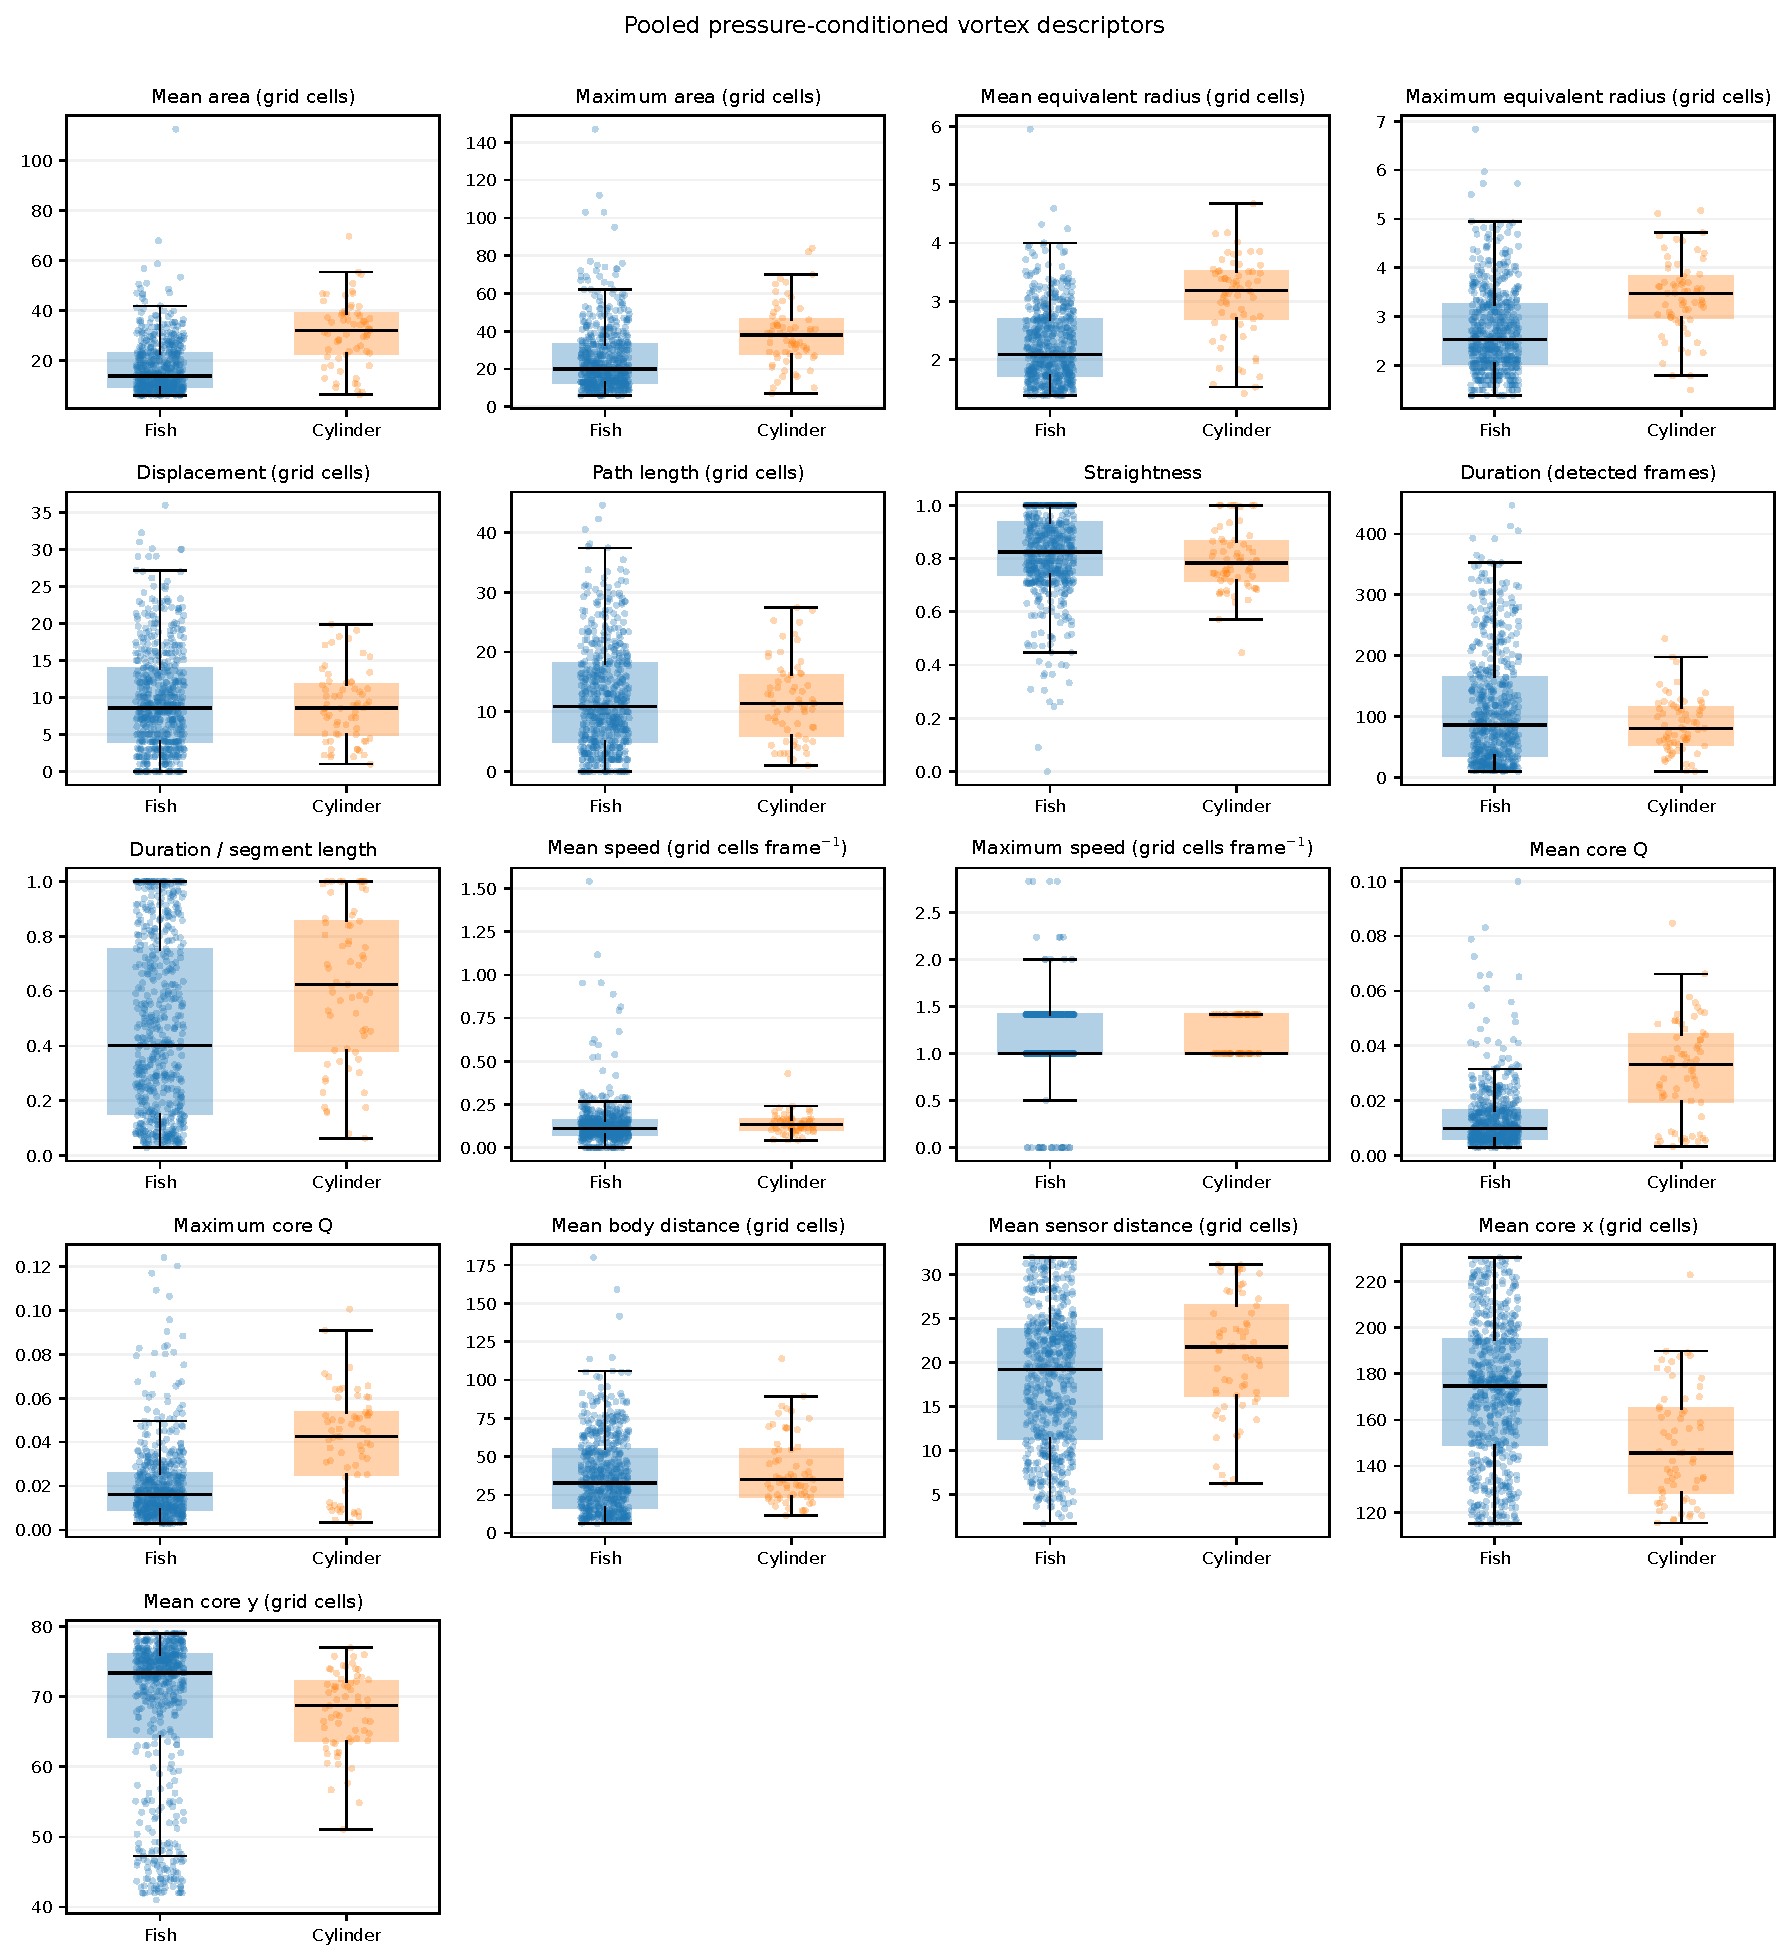
\includegraphics[width=0.94\textwidth]{supplementary_media/vortex_pooled_distributions_boai_95_thr0.99.pdf}
\caption*{\textbf{Supplementary Figure 1.} Pooled distributions of the 17 descriptors for pressure-conditioned fish-model and cylinder-model vortex-track associations. Points show individual associations. Boxes show medians and interquartile ranges, and whiskers extend to the most extreme values within 1.5 times the interquartile range.}
\end{figure}

\begin{landscape}
\begin{table}[p]
\centering
\caption*{Table S6. Equal-weight pressure-segment summaries. Track-level descriptors were averaged within each segment. Values are medians (interquartile ranges) across 88 fish-associated and 15 cylinder-associated pressure segments.}
\begin{tabular*}{0.8\linewidth}{@{\extracolsep{\fill}}lcc@{}}
\toprule
Descriptor & Fish & Cylinder \\
\midrule
Mean area (grid cells) & 15.80 (12.54--20.94) & 29.23 (19.83--33.93) \\
Maximum area (grid cells) & 23.17 (18.25--29.15) & 32.00 (27.58--42.79) \\
Mean equivalent radius (grid cells) & 2.174 (1.958--2.506) & 2.899 (2.381--3.263) \\
Maximum equivalent radius (grid cells) & 2.635 (2.327--2.896) & 3.107 (2.899--3.634) \\
Displacement (grid cells) & 10.01 (7.67--11.87) & 8.73 (8.14--10.88) \\
Path length (grid cells) & 12.05 (9.89--15.06) & 11.91 (9.98--15.01) \\
Straightness & 0.822 (0.765--0.871) & 0.767 (0.733--0.833) \\
Duration (frames) & 107.9 (83.1--143.2) & 87.6 (77.2--105.8) \\
Duration / segment length & 0.444 (0.364--0.579) & 0.607 (0.539--0.686) \\
Mean speed (grid cells frame$^{-1}$) & 0.117 (0.094--0.150) & 0.134 (0.123--0.145) \\
Maximum speed (grid cells frame$^{-1}$) & 1.119 (1.057--1.207) & 1.237 (1.101--1.303) \\
Mean core $Q$ & 0.01101 (0.00841--0.01659) & 0.02009 (0.01277--0.03807) \\
Maximum core $Q$ & 0.01750 (0.01355--0.02395) & 0.02337 (0.01611--0.04935) \\
Mean body distance (grid cells) & 37.30 (29.83--43.71) & 37.31 (26.81--45.57) \\
Mean sensor distance (grid cells) & 17.76 (15.74--19.33) & 20.35 (19.82--22.23) \\
Mean core $x$ (grid cells) & 185.81 (146.00--195.84) & 144.66 (139.77--183.13) \\
Mean core $y$ (grid cells) & 73.66 (67.23--75.37) & 67.43 (63.26--70.04) \\
Vortices per segment & 6.5 (4.0--8.0) & 4.0 (2.0--7.0) \\
Total vortex-frame occupancy & 678.0 (465.8--883.0) & 395.0 (216.5--525.5) \\
Mean simultaneous vortices & 2.79 (2.10--3.65) & 2.67 (1.31--3.81) \\
Maximum simultaneous vortices & 5.0 (4.0--6.0) & 4.0 (2.0--6.0) \\
\bottomrule
\end{tabular*}
\end{table}
\end{landscape}

\begin{figure}[p]
\centering
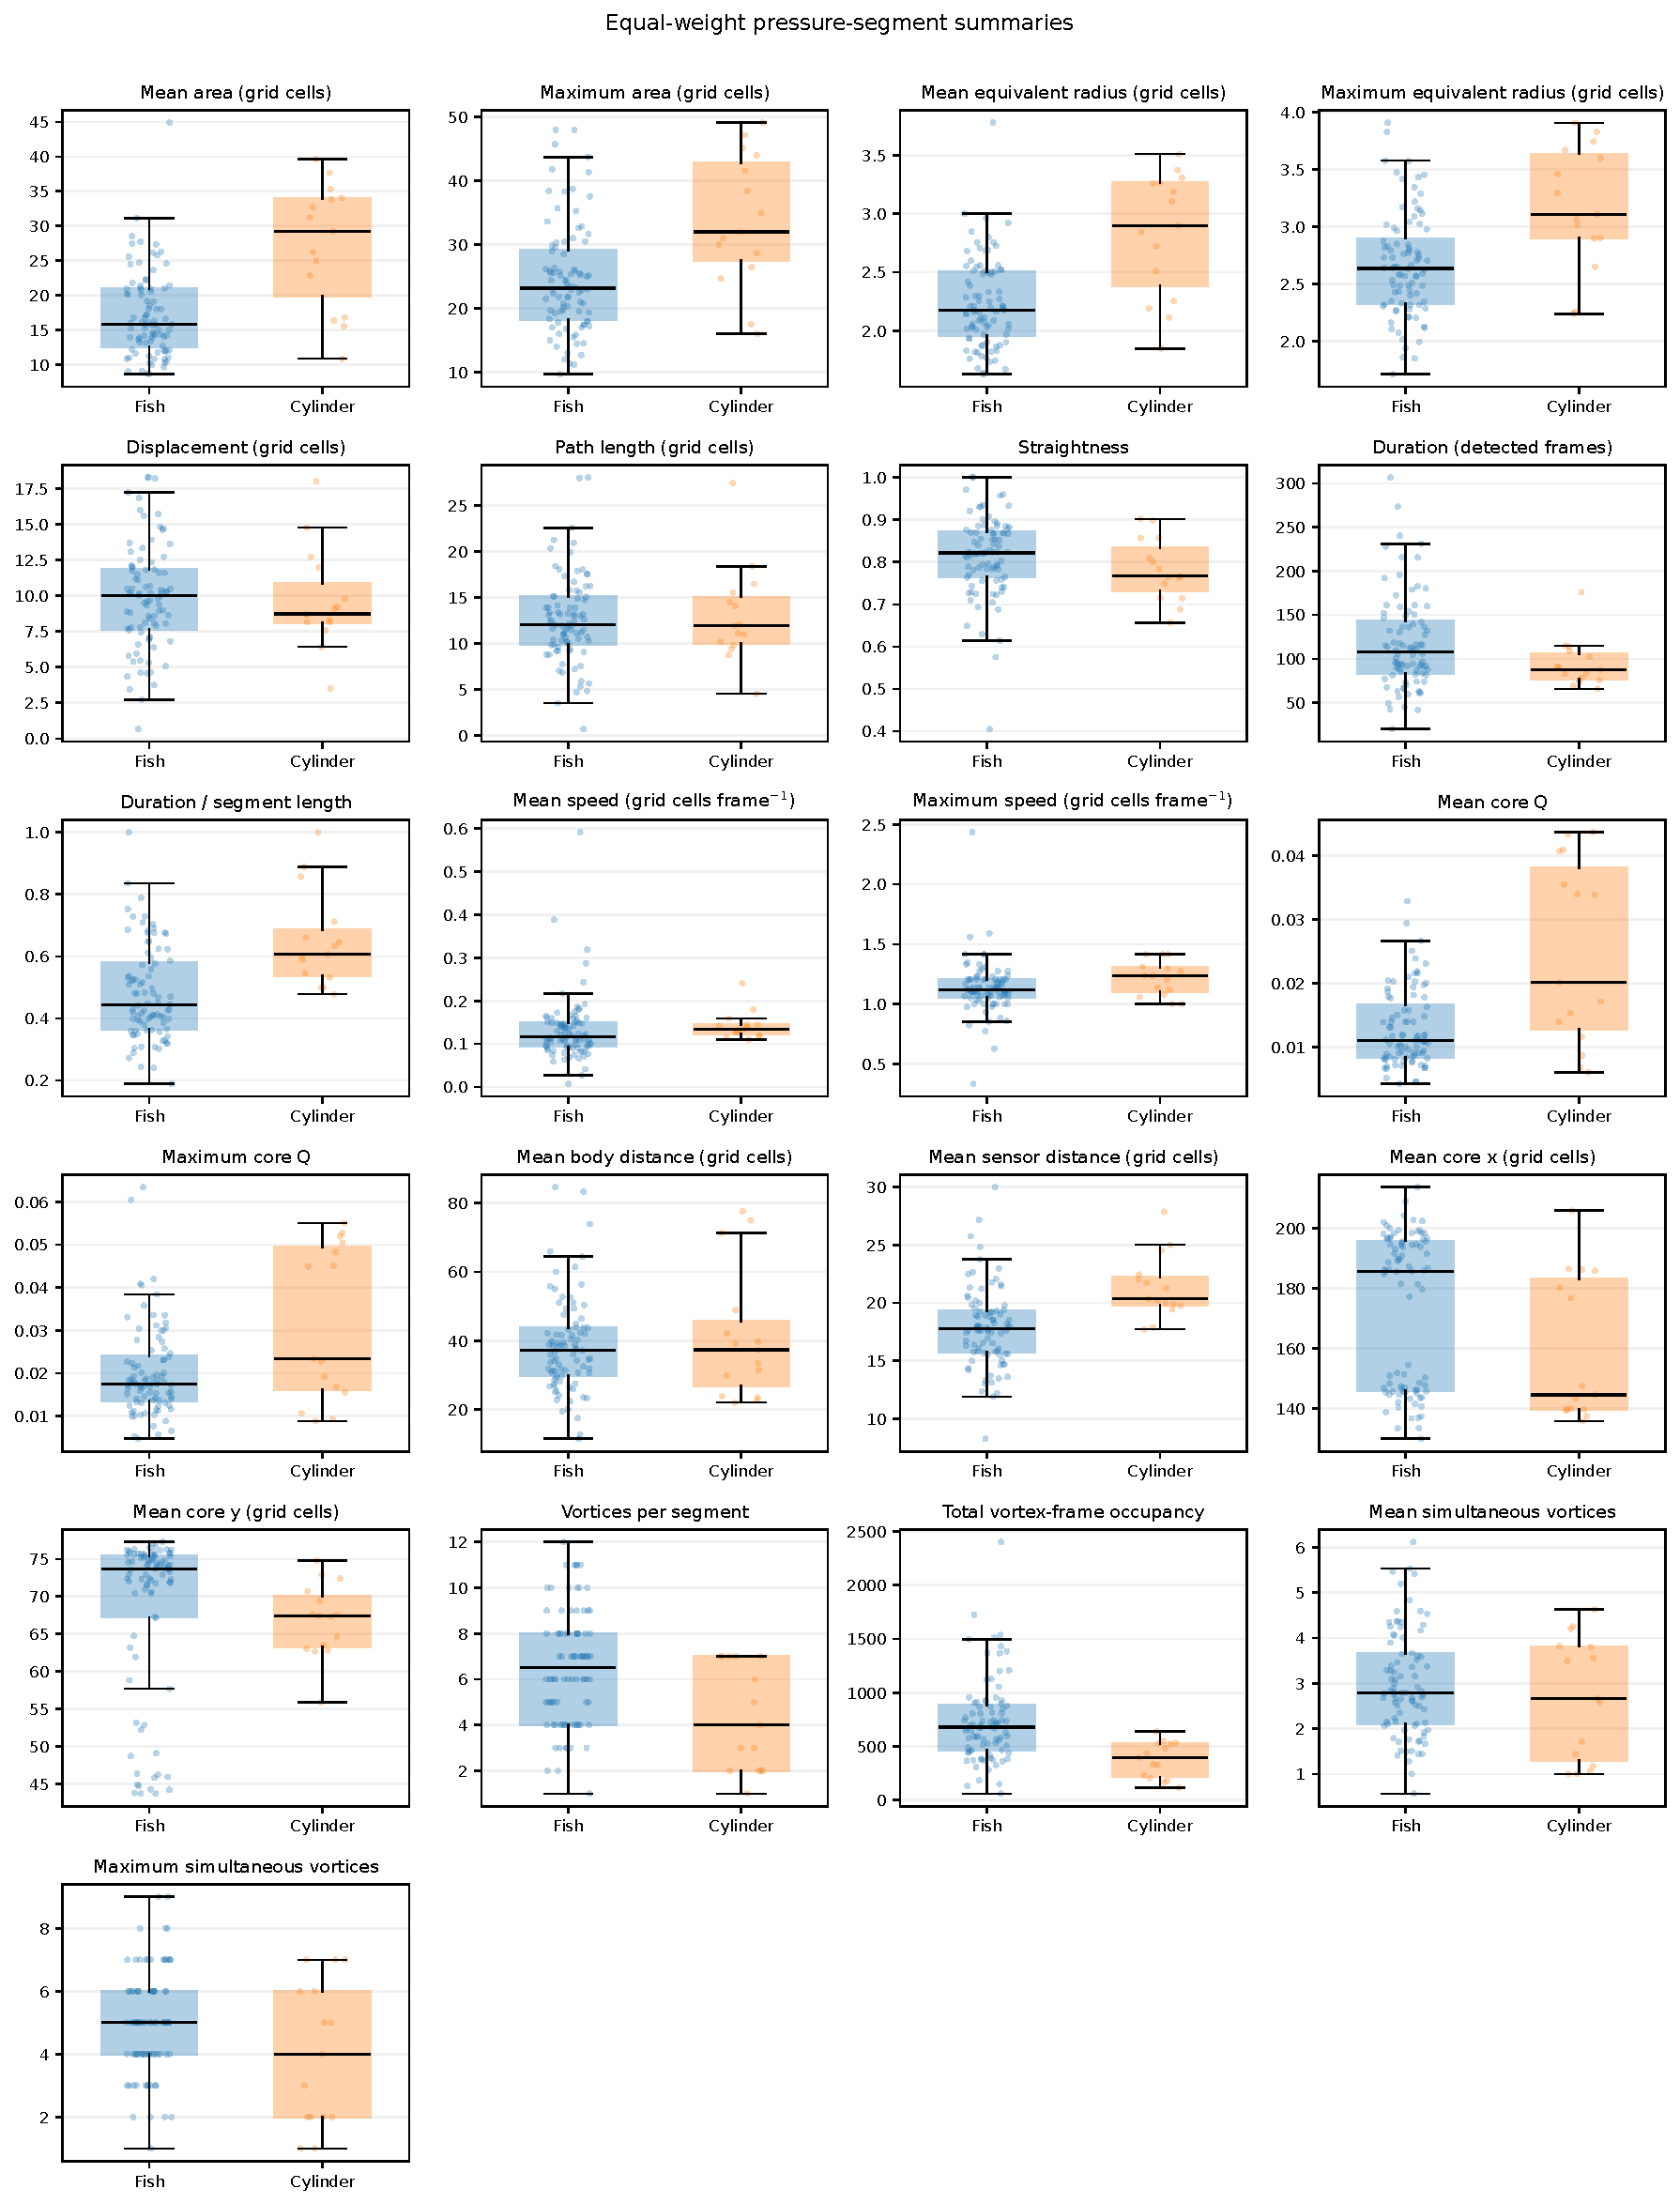
\includegraphics[width=0.94\textwidth]{supplementary_media/vortex_segment_distributions_boai_95_thr0.99.pdf}
\caption*{\textbf{Supplementary Figure 2.} Equal-weight pressure-segment distributions for the 17 track-level descriptors and four additional segment-level quantities. Points show individual pressure-segment summaries for 88 fish-associated and 15 cylinder-associated segments. Boxes show medians and interquartile ranges, and whiskers extend to the most extreme values within 1.5 times the interquartile range.}
\end{figure}

\begin{landscape}
\begin{table}[p]
\centering
\caption*{Table S7. Video-informed summaries and paired differences. Fish and cylinder columns are medians (interquartile ranges) across 21 fish-associated and 10 cylinder-associated source videos. Paired values are median cylinder-minus-fish differences (interquartile ranges) for the 10 videos represented in both groups.}
\small
\begin{tabular}{llll}
\toprule
Descriptor & Fish & Cylinder & Paired cylinder minus fish \\
\midrule
Mean area (grid cells) & 15.79 (15.01--19.16) & 25.90 (19.14--33.84) & 10.37 (4.04--13.30) \\
Maximum area (grid cells) & 23.48 (21.51--26.79) & 31.08 (25.67--42.49) & 10.67 (0.72--15.62) \\
Mean equivalent radius (grid cells) & 2.149 (2.113--2.345) & 2.798 (2.341--3.252) & 0.672 (0.219--0.728) \\
Maximum equivalent radius (grid cells) & 2.641 (2.506--2.798) & 3.097 (2.711--3.632) & 0.636 (0.056--0.819) \\
Displacement (grid cells) & 10.16 (8.75--11.51) & 8.87 (7.99--11.42) & 0.17 (-2.97--1.14) \\
Path length (grid cells) & 13.16 (11.07--13.98) & 12.50 (10.43--15.26) & 1.25 (-2.21--2.42) \\
Straightness & 0.824 (0.776--0.861) & 0.793 (0.723--0.812) & -0.052 (-0.124 to -0.015) \\
Duration (frames) & 113.9 (105.5--139.7) & 87.1 (79.8--104.2) & -25.7 (-35.4 to -21.8) \\
Duration / segment length & 0.495 (0.425--0.522) & 0.594 (0.555--0.696) & 0.108 (0.045--0.292) \\
Mean speed (grid cells frame$^{-1}$) & 0.124 (0.111--0.143) & 0.140 (0.129--0.154) & 0.017 (0.003--0.036) \\
Maximum speed (grid cells frame$^{-1}$) & 1.128 (1.083--1.184) & 1.180 (1.084--1.266) & 0.017 (-0.087--0.228) \\
Mean core $Q$ & 0.01233 (0.01050--0.01531) & 0.01854 (0.01253--0.03813) & 0.00517 (0.00133--0.02218) \\
Maximum core $Q$ & 0.01930 (0.01708--0.02278) & 0.02424 (0.01642--0.04908) & 0.00531 (-0.00270--0.02902) \\
Mean body distance (grid cells) & 35.95 (34.35--40.36) & 38.05 (25.68--46.60) & -0.37 (-11.12--9.05) \\
Mean sensor distance (grid cells) & 17.18 (16.42--18.98) & 21.22 (19.93--22.42) & 2.26 (-0.03--4.03) \\
Mean core $x$ (grid cells) & 175.67 (165.93--180.27) & 151.58 (140.80--181.55) & -5.07 (-29.41--4.96) \\
Mean core $y$ (grid cells) & 72.31 (65.53--74.61) & 67.36 (64.60--69.91) & 1.23 (-6.24--7.30) \\
Vortices per segment & 6.5 (5.8--7.4) & 3.7 (2.2--6.1) & -2.8 (-4.1 to -1.0) \\
Total vortex-frame occupancy & 707.4 (534.5--839.5) & 395.5 (216.8--514.4) & -304.2 (-491.9 to -235.8) \\
Mean simultaneous vortices & 2.94 (2.57--3.32) & 2.57 (1.38--3.79) & -0.31 (-1.60--0.72) \\
Maximum simultaneous vortices & 5.2 (4.3--5.6) & 3.5 (2.0--5.8) & -1.5 (-2.8--0.5) \\
\bottomrule
\end{tabular}
\end{table}
\end{landscape}

\clearpage

\section*{S9. Results for 75\% and 99\%}

\begin{figure}[htbp]
\centering
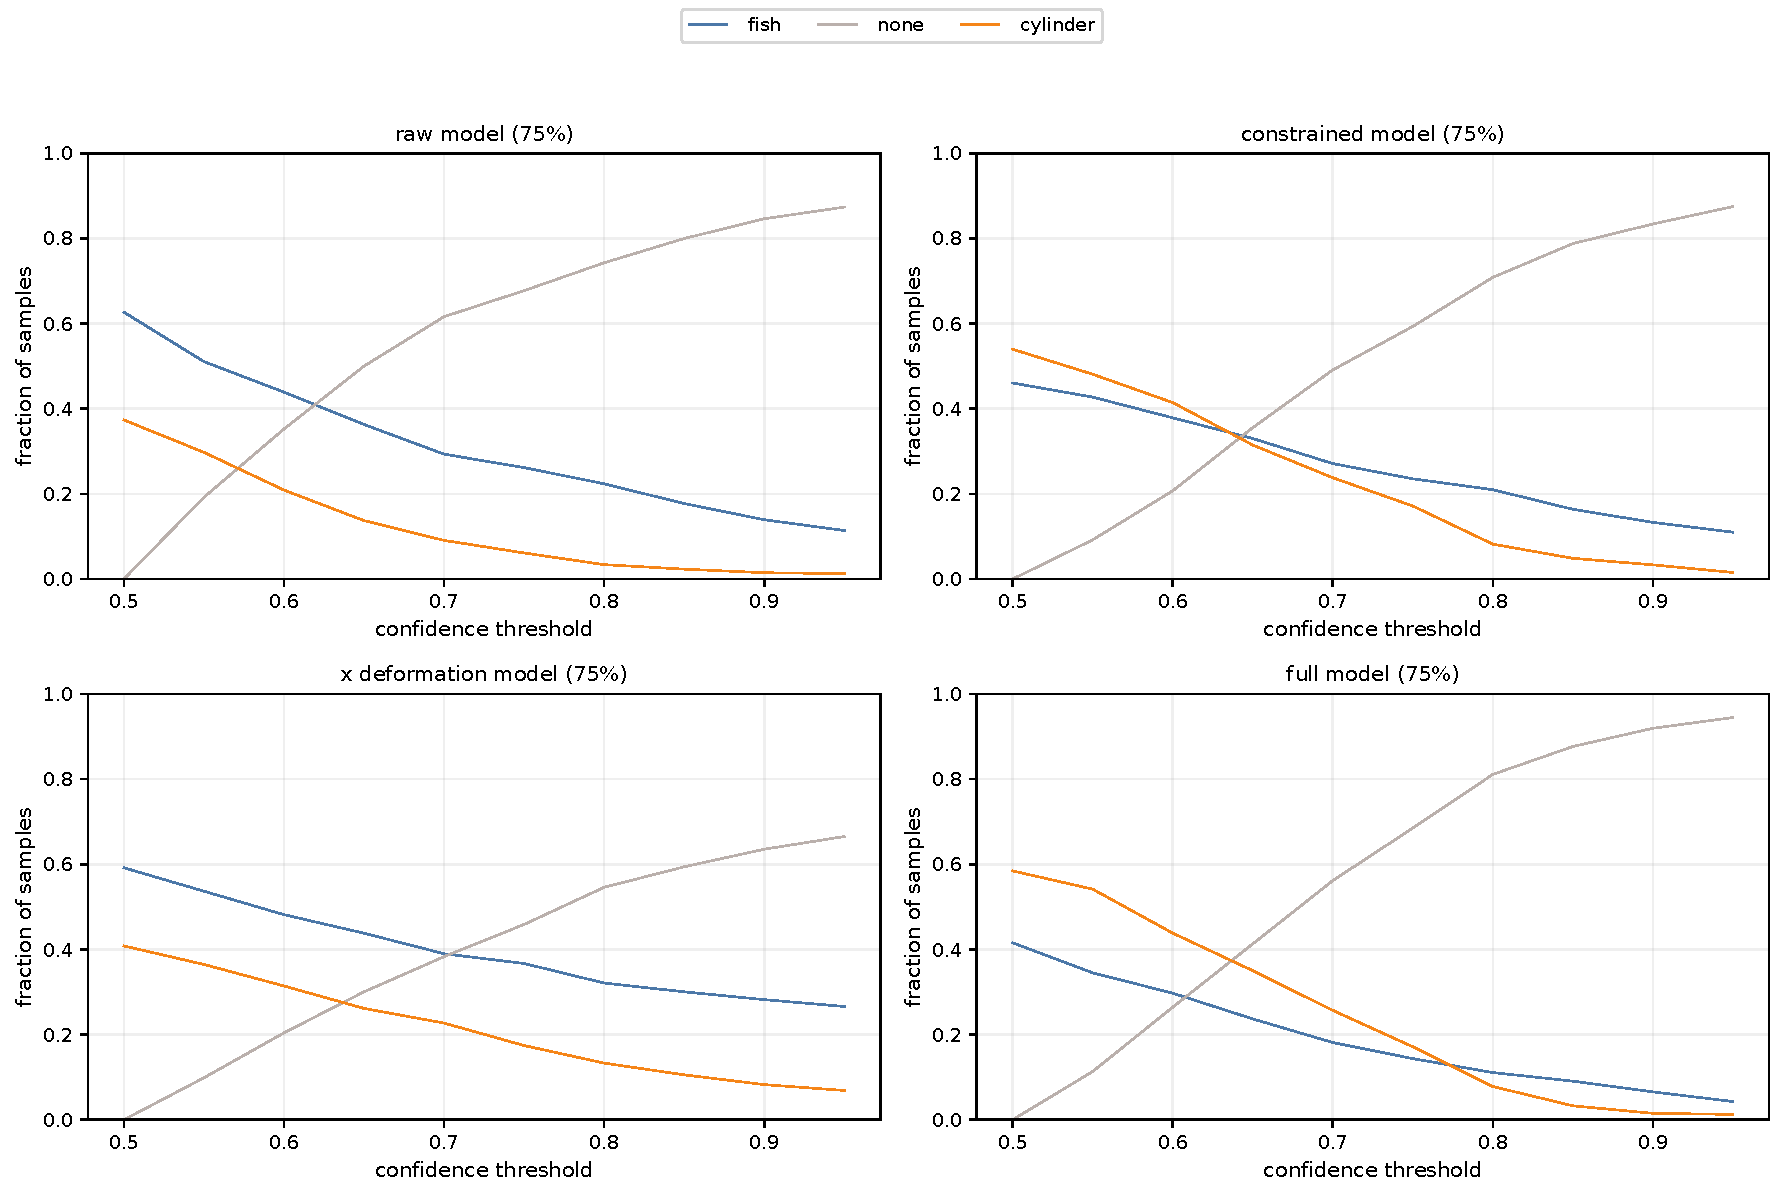
\includegraphics[width=1\textwidth]{supplementary_media/real_pressure_threshold_curves_75.pdf}
\caption*{\textbf{Supplementary Figure 3.} Fractions of measured pressure-signal segments classified as fish-like, cylinder-like or undetermined when 75\% of variance was retained. Across most configurations, measured signals were more frequently associated with the fish-shaped model than with the cylinder surrogate.}
\end{figure}

\begin{figure}[htbp]
\centering
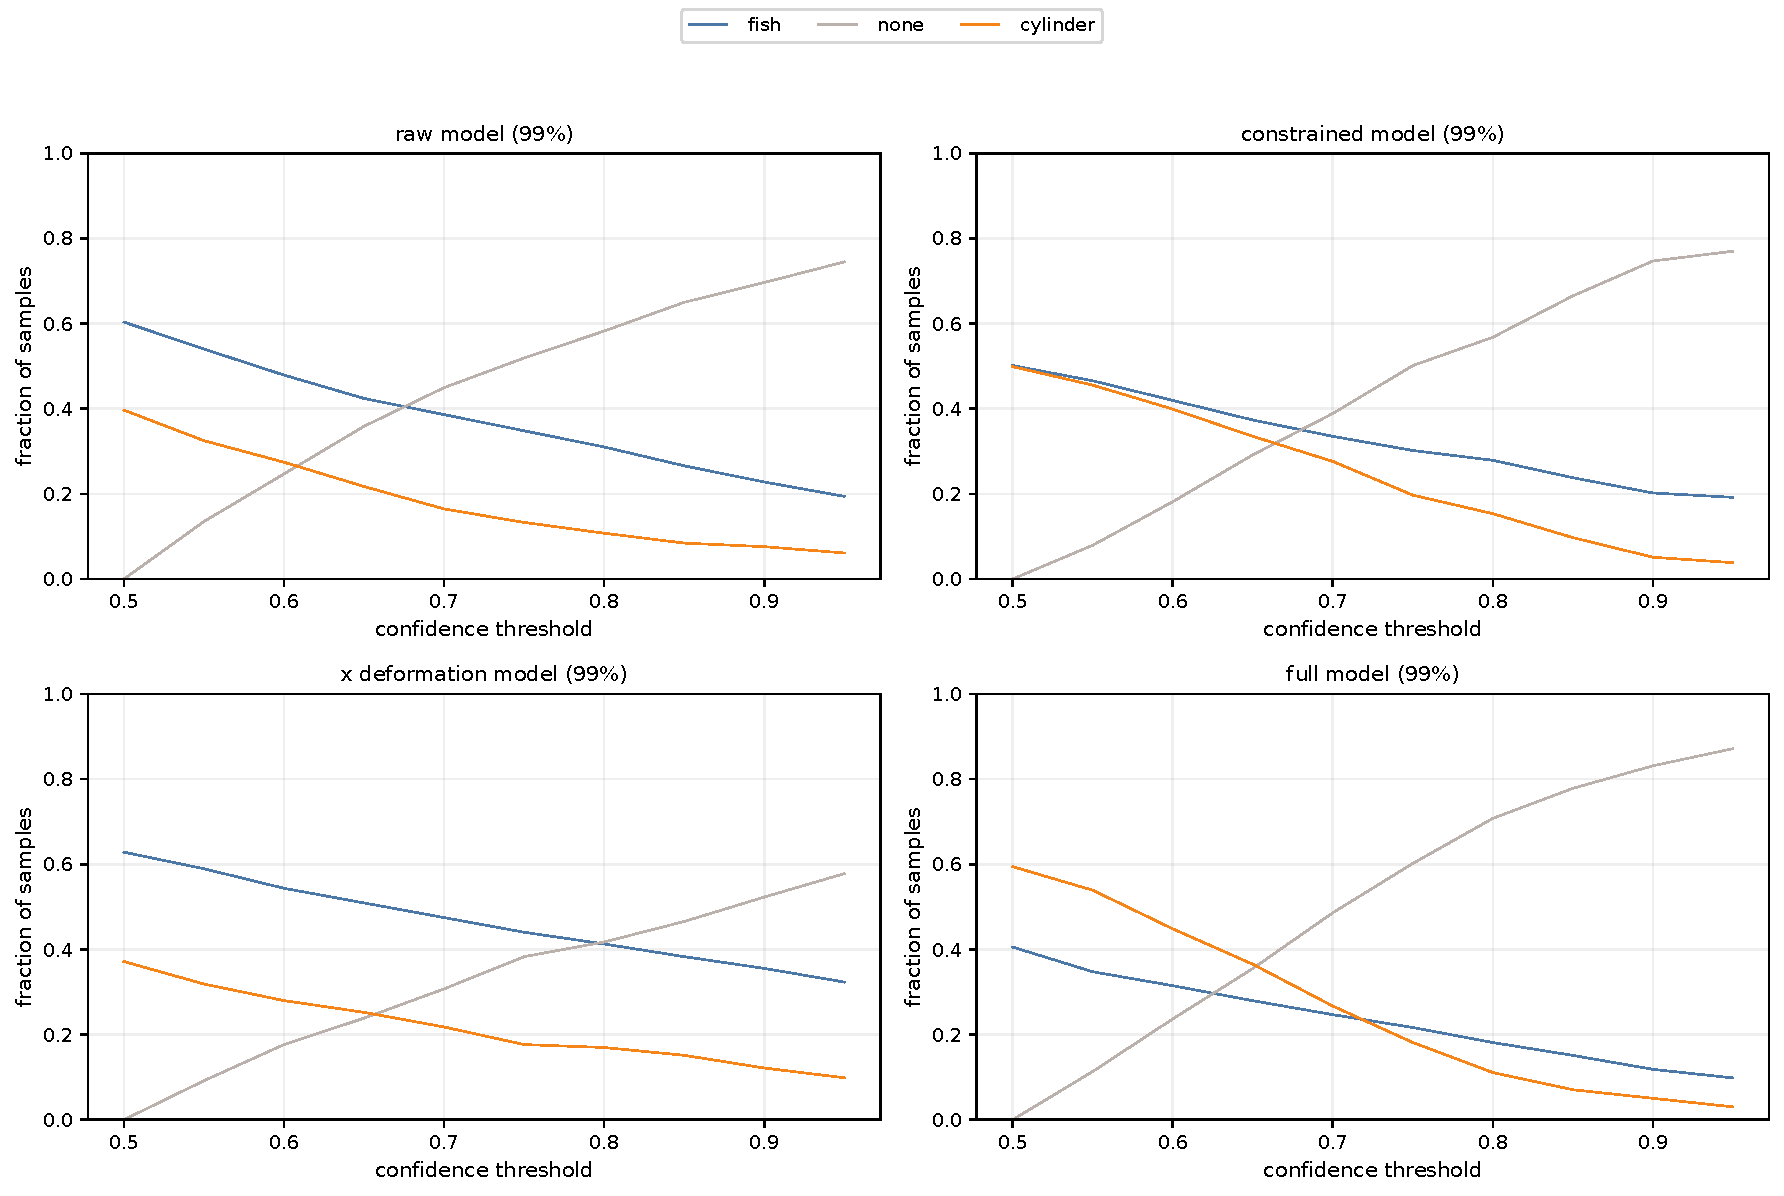
\includegraphics[width=1\textwidth]{supplementary_media/real_pressure_threshold_curves_99.pdf}
\caption*{\textbf{Supplementary Figure 4.} Fractions of measured pressure-signal segments classified as fish-like, cylinder-like or undetermined when 99\% of variance was retained. Across most configurations, measured signals were more frequently associated with the fish-shaped model than with the cylinder surrogate.}
\end{figure}

\clearpage

\section*{S10. Body-distance sensitivity across model variants}

\begin{figure}[htbp]
\centering
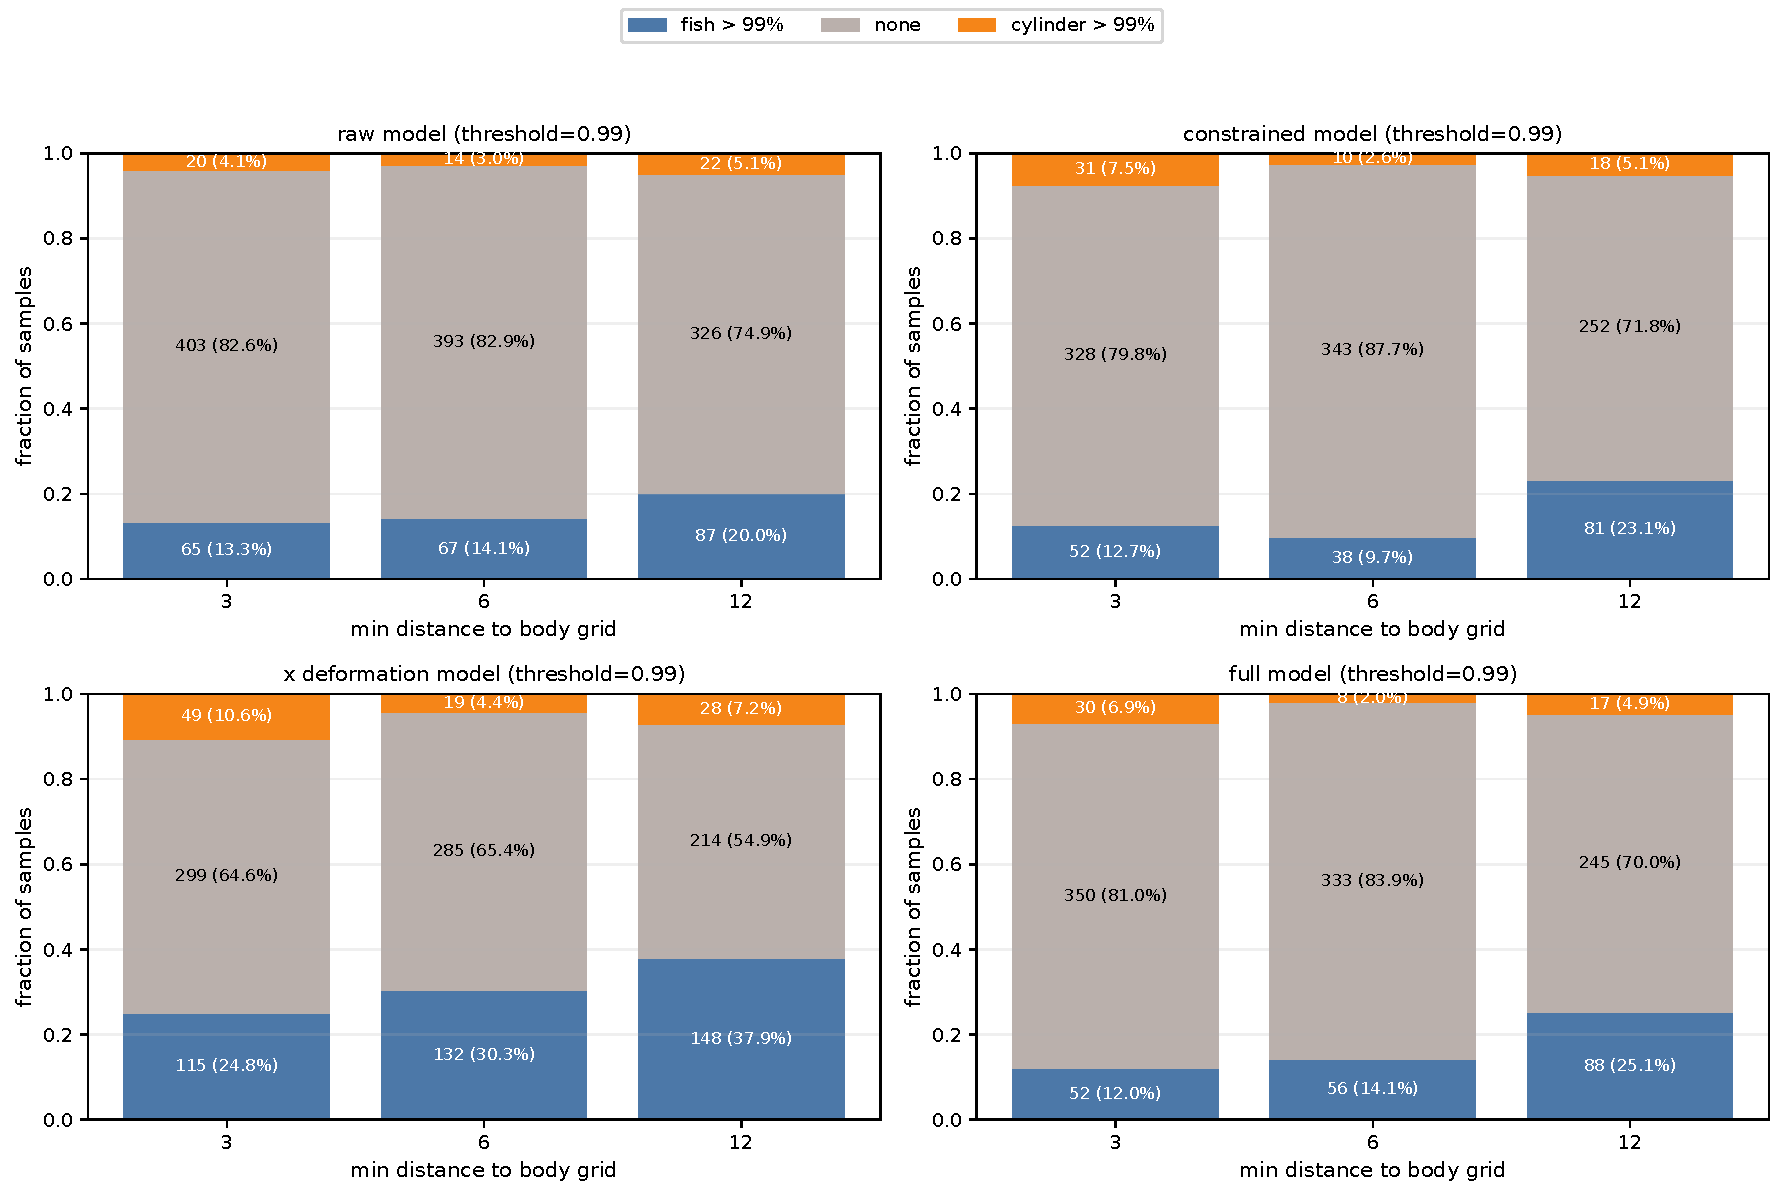
\includegraphics[width=1\textwidth]{supplementary_media/paper_ready_distribution_min_distance_all_models.pdf}
\caption*{\textbf{Supplementary Figure 5.} Effect of the minimum vortex-to-body distance on measured pressure classification for the raw, size-constrained, x-deformation and full model variants at 0.99 confidence. The x-axis gives the exclusion threshold in 1 mm simulation-grid cells. Blue, grey and orange represent fish-like, undetermined and cylinder-like fractions, respectively. Across the four variants, stronger exclusion of near-body vortices generally increased the fish-like fraction.}
\end{figure}

\end{document}
